\documentclass{beamer}

\usepackage{shyne}

% Theme settings
\setbeamertemplate{navigation symbols}{}

\usetheme{Madrid}
\usefonttheme{structurebold}

\AtBeginSection[]
{ 	\begin{frame}{}

	{
	\usebeamerfont{frametitle}
	\begin{beamercolorbox}
		[wd={\textwidth}, center, sep=.2in, rounded=true, shadow=true]
		{frametitle}
	Chapter \thesection\\  \secname 
	\end{beamercolorbox}
	}
	
	\end{frame} 
}

\AtBeginSubsection[]
{ 	\begin{frame}{}

	{
	\usebeamerfont{frametitle}
	\begin{beamercolorbox}
		[wd={\textwidth}, center, sep=.2in, rounded=true, shadow=true]
		{frametitle}
	Section \thesection .\thesubsection\\  \subsecname 
	\end{beamercolorbox}
	}
	
	\end{frame} 
}

\title[Chapter 2]{Stat 201: Statistics I\\ Chapter 2 }
\author[M. Shyne]{}
\institute[Metro State]{
\includegraphics[width=1.75in]{../images/metro_logo}}
\date[date]{date
\\ \bigskip \bigskip 
\includegraphics[width=.4in]{../images/cc_big}}


\begin{document}

\frame{\titlepage}

% Chapter 2
\setcounter{section}{1}
\section{Summarizing and Graphing Data}

% Section 2.1
\subsection{Frequency Distributions for Organizing and Summarizing Data}

\begin{frame}
\frametitle{Frequency distributions}

\begin{block}{}
\large
A \bt{frequency} is the number of times a particular value occurs in a set of data, i.e. the count.
\end{block}
\pause
\begin{block}{}
\large
A \bt{frequency distribution} (or \bt{frequency table}) summarizes a set of data by listing the frequencies of data in categories or classes (groups).
\begin{itemize}
\item For categorical data, the categories are simply the possible values of the data.
\item For quantitative data, the classes are usually ranges of possible values.
\end{itemize}
\end{block}
\end{frame}

\begin{frame}
\frametitle{Frequency distribution for categorical data}

\begin{exampleblock}{Example}
\bt{Favorite kind of taco} = \{Chicken, Fish, Fish, Veggie, Chicken, Beef \}
\pause
\begin{center}
\begin{tabular}{c | c}
Kind of taco & Frequency\\
\hline
Beef & 1\\
Chicken & 2\\
Pork & 0\\
Fish & 2\\
Veggie & 1
\end{tabular}
\end{center}
\end{exampleblock}

\end{frame}

\begin{frame}
\frametitle{Frequency distribution for quantitative data}

\begin{exampleblock}{Example}
\bt{Tacos eaten} = \{3, 0, 17, 6, 4, 3, 5 \}
\pause
\begin{center}
\begin{tabular}{c | c}
Number of tacos eaten & Frequency\\
\hline
0 - 4 & 4\\
5 - 9 & 2\\
10 - 14 & 0\\
15 -20 & 1
\end{tabular}
\end{center}
\end{exampleblock}

\end{frame}

\begin{frame}
\frametitle{Relative frequency}

\begin{block}{}
\large
\bt{Relative frequency} is the proportion (fraction) of the whole data set that resides in each category or class. When expressed as a percent it is called \bt{percentage frequency}.
\end{block}
\pause
\begin{block}{}
To calculate: For each class,
\[\text{Relative frequency} = \frac{\text{class frequency}}{\text{total count}}\]
\[\text{Percentage frequency} = \frac{\text{class frequency}}{\text{total count}} \times 100\]
\end{block}

\end{frame}

\begin{frame}
\frametitle{Relative frequency example}

\begin{exampleblock}{Example}

\begin{center}
\begin{tabular}{c | c | c | c}
Tacos eaten & Frequency & Relative & Percentage\\
\hline
0 - 4 & 4 & 0.5714 & 57.14 \%\\
5 - 9 & 2 & 0.2857 & 28.57 \%\\
10 - 14 & 0 & 0 & 0 \%\\
15 -20 & 1 & 0.1428 & 14.28 \%\\
\hline
Total & 7 & 1 & 100 \%
\end{tabular}
\end{center}
\end{exampleblock}

\end{frame}

\begin{frame}
\frametitle{Cumulative frequency}

\begin{block}{}
\large
\bt{Cumulative frequency} is the frequency for a class and \emph{all previous classes}.
\end{block}
\pause
\begin{exampleblock}{Example}

\begin{center}
\begin{tabular}{c | c | c }
Tacos eaten & Frequency & Cumulative\\
\hline
0 - 4 & 4 & 4\\
5 - 9 & 2 & 6\\
10 - 14 & 0 & 6\\
15 -20 & 1 & 7\\
\end{tabular}
\end{center}
\end{exampleblock}

\end{frame}

\begin{frame}
\frametitle{Normal distributions}

\begin{block}{}
\large
A \bt{normal distribution} can be identified from a frequency table that has the following characteristics:
\begin{itemize}
\item The frequencies start low, increase to a high point and then decrease to low frequencies at the end
\item The frequencies are approximately symmetric around the high point.
\end{itemize}
\end{block}
\end{frame}

\begin{frame}
\frametitle{Normal distributions, example}

\begin{exampleblock}{Example}
\begin{columns}[c]
\column{.5\textwidth}
\begin{center}
\begin{tabular}{c|c}
\multicolumn{2}{c}{\emph{Normal}}\\
IQ & Frequency\\
\hline
80 - 89 & 1 \\
90 - 99 &  5\\
100 - 109 & 11\\
110 - 119 & 10\\
120 - 129 &  4\\
130 - 139 & 2

\end{tabular}
\end{center}
\column{.5\textwidth}
\begin{center}
\begin{tabular}{c|c}
\multicolumn{2}{c}{\emph{Not normal}}\\
IQ & Frequency\\
\hline
80 - 89 & 2\\
90 - 99 &  9 \\
100 - 109 &  13\\
110 - 119 & 4 \\
120 - 129 & 3\\
130 - 139 & 1

\end{tabular}
\end{center}

\end{columns}
\medskip

\end{exampleblock}

\end{frame}

\begin{frame}
\frametitle{Gaps in frequency tables}
\begin{block}{}
\large
A \bt{gap} of frequencies in a table indicates that the data probably come from two different populations.
\end{block}
\pause
\begin{block}{}
\large
The converse is not necessarily true. Data from two different populations might not display a gap.
\end{block}
\pause
\begin{exampleblock}{Example}
\begin{itemize}
\item Pennies made before 1983 are 95\% copper and 5\% zinc.
\item Pennies made after 1983 are 2.5\% copper and 97.5\% zinc. 
\end{itemize}
\end{exampleblock}
\end{frame}

\begin{frame}{Gaps in frequency tables, example}

\begin{exampleblock}{Example, cont.}
\begin{center}
\begin{tabular}{c|c}
Weight (g) of penny & Frequency\\
\hline
2.40 - 2.49 & 18 \\
2.50 - 2.59 & 19\\
2.60 - 2.69 & 0\\
2.70 - 2.79 & 0\\
2.80 - 2.89 & 0\\
2.90 - 2.99 & 2\\
3.00 - 3.09 & 25\\
3.10 - 3.19 & 8\\
\end{tabular}
\end{center}
\end{exampleblock}
\end{frame}

% Section 2.2
\subsection{Histograms}

\begin{frame}{Histograms}
\begin{block}{}
\large
A \bt{histogram} is a graphical representation of a frequency distribution of quantitative data. This allows the distribution of the data to be more easily visualized.
\end{block}

\begin{center}
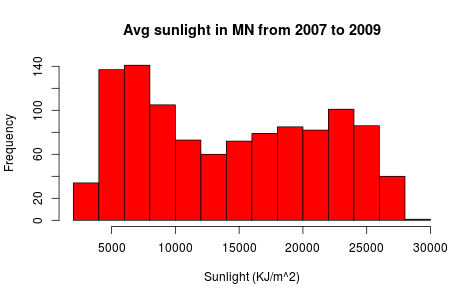
\includegraphics[width=3.8in]{../images/ch02_sunlight_hist}
\end{center}
\end{frame}

\begin{frame}{Properties of histograms}
\begin{block}{}
\begin{itemize}
\item A graph of bars of equal width drawn adjacent to each other.
\pause
\item The horizontal scale (x-axis) represents values of the quantitative data. Each bar represents a class, or range of values, from a frequency table. 
\pause
\item The vertical scale (y-axis) represents frequency (counts), or proportions (relative frequency) or percentages (percentage frequency).
\pause
\item The number of bars is largely an aesthetic choice. There should be enough bars to adequately show the shape of the distribution, but too many can make a ``busy" graph that's hard to read. Most software will automatically choose the number of bars.
\end{itemize}
\end{block}
\end{frame}

\begin{frame}{Histograms and normal distributions}
\begin{block}{}
Recall, a \bt{normal distribution} can be identified from a frequency table that has the following characteristics:
\begin{itemize}
\item The frequencies start low, increase to a high point and then decrease to low frequencies at the end
\item The frequencies are approximately symmetric around the high point.
\end{itemize}
\end{block}
\pause
\begin{block}{}
Graphically, normal distributions are commonly known as ``bell curves". Histograms can be used to recognize when data follows a normal distribution.
\end{block}
\end{frame}

\begin{frame}{Histograms and normal distributions, examples}

{\centering
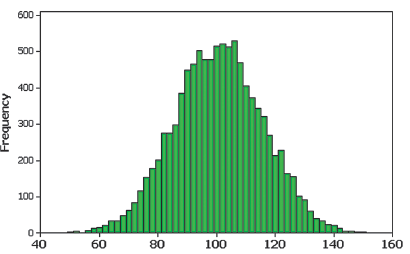
\includegraphics[width=4in]{../images/ch02_hist_norm}
\par}
\bigskip
\pause
\begin{block}{}
\centering \large Normal
\end{block}
\end{frame}

\begin{frame}{Histograms and normal distributions, examples}

{\centering
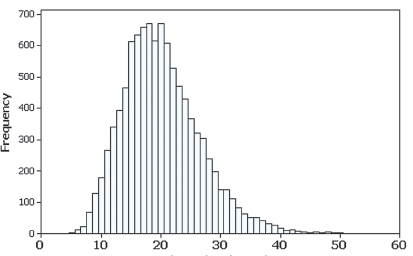
\includegraphics[width=4in]{../images/ch02_hist_rskew}
\par}
\bigskip
\pause
\begin{block}{}
\centering \large Right skewed
\end{block}
\end{frame}

\begin{frame}{Histograms and normal distributions, examples}

{\centering
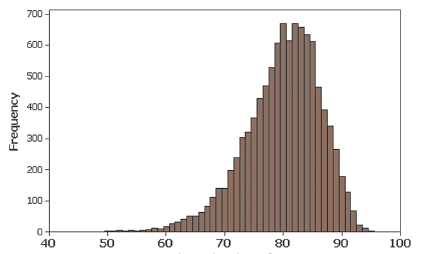
\includegraphics[width=4in]{../images/ch02_hist_lskew}
\par}
\bigskip
\pause
\begin{block}{}
\centering \large Left skewed
\end{block}
\end{frame}

\begin{frame}{Histograms in StatCrunch}
\begin{block}{}
\begin{itemize}
\item Graph $\to$ Histogram
\item Select column that contains data for histogram
\item Optional: Select type of histogram. This will adjust y-axis scale.
\item Optional: Set ``Bin: Width". This will determine number of bars displayed.
\item Click ``Compute!"
\end{itemize}
\end{block}

\begin{alertblock}{Note}
StatCrunch expects raw data for generating histograms. It won't work with data in frequency tables. To approximate a histogram using a frequency table, use a bar graph (see next section).
\end{alertblock}
\end{frame}

% Section 2.3
\subsection{Graphs that Enlighten and Graphs that Deceive}

\begin{frame}{Types of graphs}

\begin{block}{}
\large
There are many types of graphs. Deciding which to use depends on the type of data involved and the message to be delivered.
\end{block}
\end{frame}

\begin{frame}{Types of graphs: dotplots}
\begin{block}{}
A \bt{dotplot} is similar to a histogram. 
\begin{itemize}
\item The x-axis represents values of the quantitative data
\item Instead of bars, a dot is placed for each instances of a value
\end{itemize}
\end{block}
\bigskip
{\centering
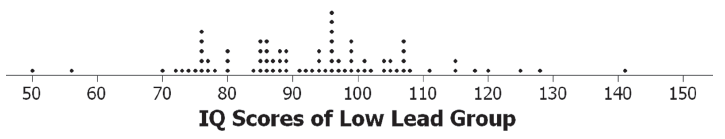
\includegraphics[width=4in]{../images/ch02_dotplot}
\par}
\end{frame}


\begin{frame}{Types of graphs: stem-and-leaf plots}
\begin{block}{}
A \bt{stem-and-leaf plot} is also used display frequencies of quantitative data
\begin{itemize}
\item Each numeric value is separated into two parts, the leftmost digits (the stem) and the last digit (the leaf). For example, 142 $\implies$ 14 and 2.
\item Each stem is arranged vertically on the left side of the graph.
\item Every leaf belonging to a stem is listed to the right, in numeric order.
\end{itemize}
\end{block}
\pause

\begin{exampleblock}{Example}
\begin{columns}
\column{.5\textwidth}
\centering
\begin{tabular}{c c c | c}
Value & $\implies$ & Stem & Leaf\\
142 && 14 & 2\\
146 && 14 & 6\\
138 && 13 & 8\\
143 && 14 & 3
\end{tabular}
\pause
\column{.5\textwidth}
\centering
Stem-and-leaf plot\\

\begin{tabular}{c|l}
13 & 8\\
14 & 2 3 6
\end{tabular}
\end{columns}
\end{exampleblock}
\end{frame}

\begin{frame}{Stem-and-leaf plot, example}
\bigskip
{\centering
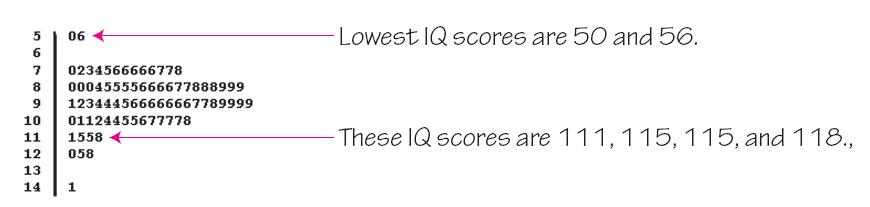
\includegraphics[width=4.25in]{../images/ch02_stem}
\par}

\end{frame}

\begin{frame}{Types of graphs: bar graph}
\begin{block}{}
A \bt{bar graph} displays frequencies of categorical data.
\begin{itemize}
\item The horizontal scale (x-axis) represents values of the categorical data.
\item The vertical scale (y-axis) represents frequencies (or proportions or percentages).
\item Often, but not always, bars are drawn with a gap between values.
\end{itemize}
\end{block}
\end{frame}

\begin{frame}{Bar graph, example}
\bigskip
{\centering
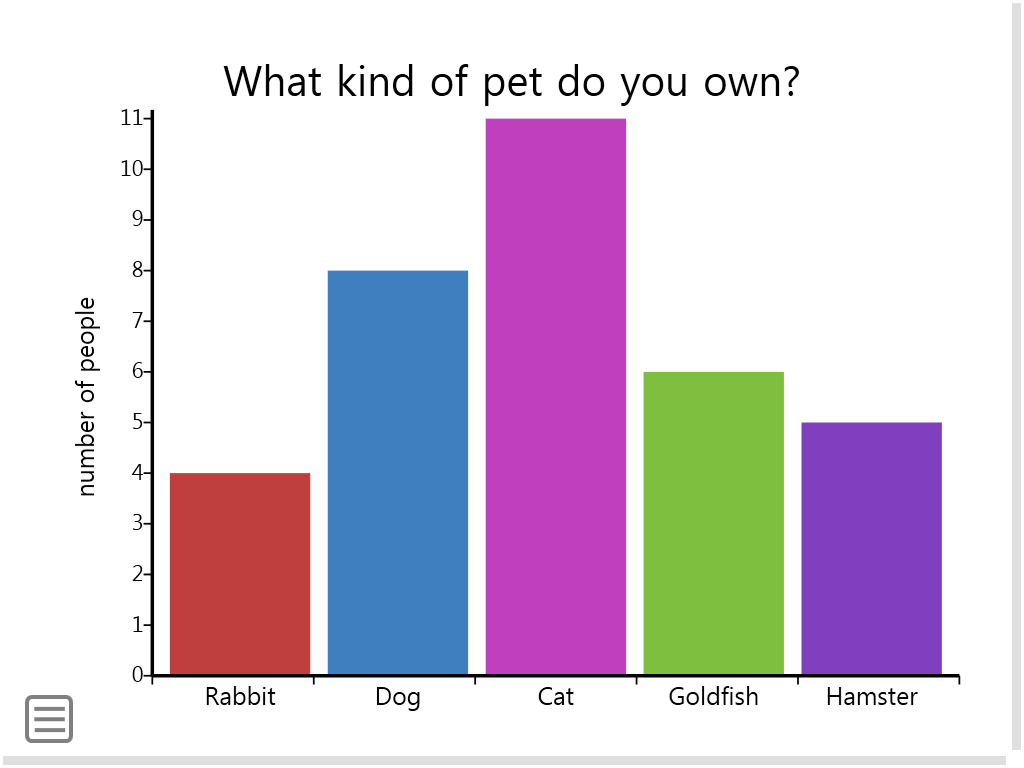
\includegraphics[width=4in]{../images/ch02_bar}
\par}

\end{frame}

\begin{frame}{Types of graphs: Pareto charts}

\begin{block}{}
A \bt{Pareto chart} is very similar to a bar graph, except the bars are arranged from most frequent to least, left to right.
\begin{itemize}
\item Can be confusing if used with ordinal data.
\end{itemize} 
\end{block}

\bigskip
{\centering
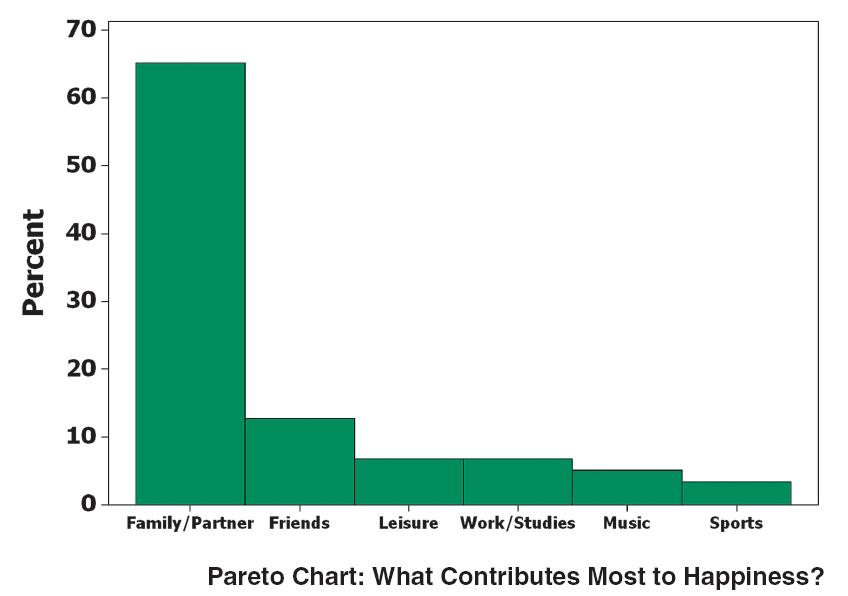
\includegraphics[width=3in]{../images/ch02_pareto}
\par}

\end{frame}

\begin{frame}{Types of graphs: pie charts}

\begin{block}{}
A \bt{pie chart} displays relative frequencies of categorical data as ``slices" of a whole circle. The ``slices'' must be labelled or distinguished by color.
\end{block}

\bigskip
{\centering
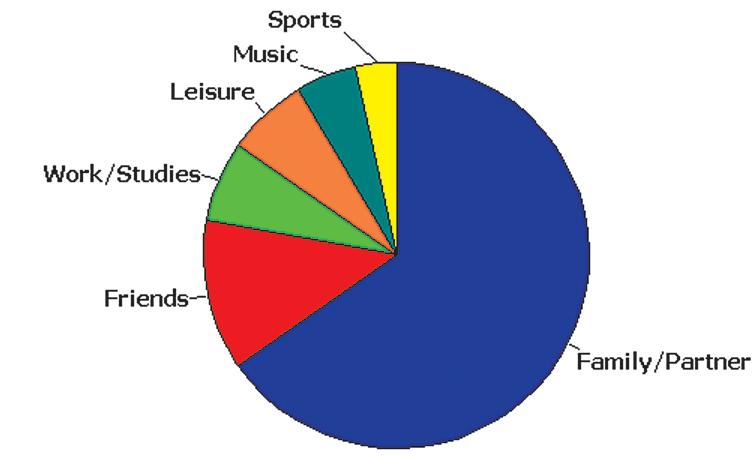
\includegraphics[width=3.5in]{../images/ch02_pie}
\par}

\end{frame}

\begin{frame}{Types of graphs: scatterplots}
\begin{block}{}
A \bt{scatterplot} displays the relationship between paired quantitative variables.
\begin{itemize}
\item The x-axis represents one variable and the y-axis the other.
\item A dot (or other symbol) for each data pair is placed at the appropriate x and y values.
\end{itemize} 
\end{block}

\bigskip
{\centering
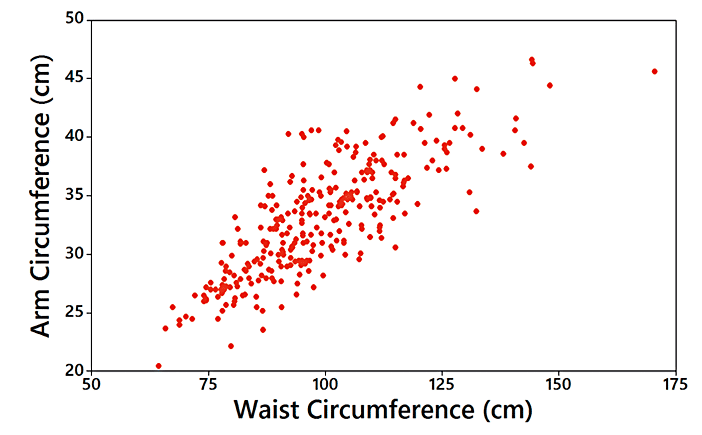
\includegraphics[width=2.9in]{../images/ch02_scatter}
\par}

\end{frame}

\begin{frame}{Scatterplots and correlation}
\begin{block}{}
\large
A question that can be answered with a scatterplot is whether there is an association or correlation between variables.  
\end{block}
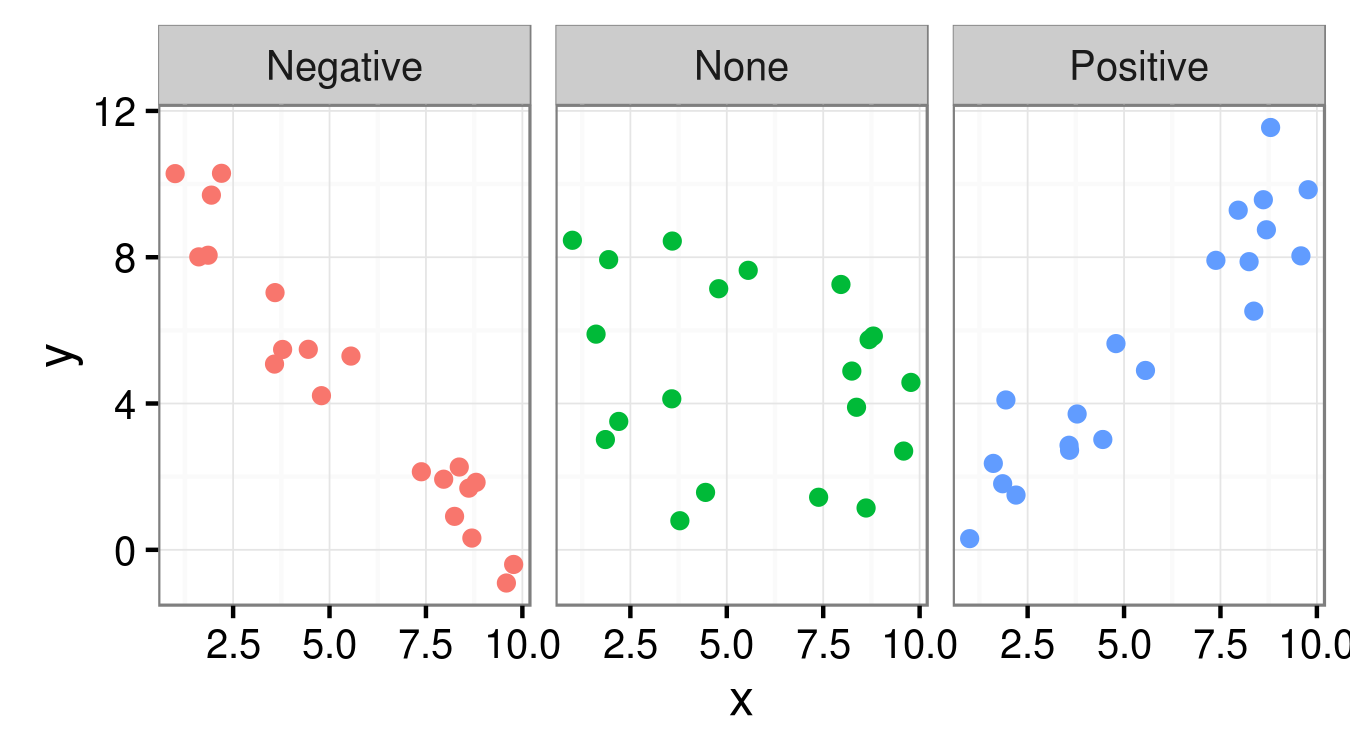
\includegraphics[width=4.5in]{../images/ch02_scatter_cor}
\end{frame}

\begin{frame}{Types of graphs: time series}
\begin{block}{}
A graph of paired quantitative data where one variable represents time is called a \bt{time series}. It is much like a scatterplot, except\ldots
\begin{itemize}
\item The x-axis always represents the time variable.
\item Often a line is drawn between the points.
\end{itemize}
\end{block}
\bigskip
{\centering
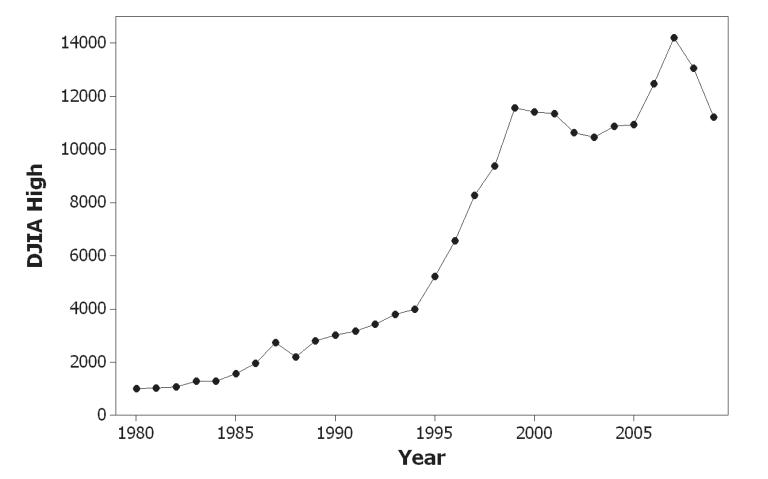
\includegraphics[width=3in]{../images/ch02_timeseries}
\par}

\end{frame}

\begin{frame}{Graphs in StatCrunch}
\begin{block}{Dotplots and stem-and-leaf plots}
\begin{itemize}
\item Graph $\to$ Dotplot or Stem and Leaf
\item Select column that contains the data to be graphed
\item Click ``Compute!"
\end{itemize}
\end{block}

\begin{block}{Bar plots and pie charts}
\begin{itemize}
\item Graph $\to$ Bar Plot or Pie Chart $\to$ With Summary
\item Select the column containing category names
\item Select the column containing category counts
\item Click ``Compute!"
\end{itemize}
\end{block}


\begin{block}{Pareto charts}
Follow steps for bar chart, except...
\begin{itemize}
\item Under ``Order by" select ``Count descending"
\end{itemize}
\end{block}
\end{frame}

\begin{frame}{Graphs in StatCrunch}
\begin{block}{Scatterplots and time series plots}
\begin{itemize}
\item Graph $\to$ Scatter plot
\item Select column that contains the data for the x-axis (time variable for time series plots)
\item Select column that contains the data for the y-axis
\item For time series plots, under ``Display" select lines (shift-click to select both points and lines)
\item Click ``Compute!"
\end{itemize}
\end{block}

\end{frame}


\begin{frame}{Graphs that deceive}
\begin{block}{}
There are two types of bad graphs:
\begin{itemize}
\item Sometimes a graph is factually incorrect, whether because of errors in the data or a mistake in creating the graph. This is often difficult to detect without access to the original data.
\item Sometimes graphs are technically correct, but designed to give a false impression of the data. Part of being a critical consumer of statistics is learning to recognize these misleading graphs.
\end{itemize}
\end{block}
\end{frame}

\begin{frame}{Misleading graphs: non-zero axis}
\begin{block}{}
A \bt{non-zero axis} is when one of the axis has a scale which does not include zero. This can make the relative sizes of the graph items to be distorted, especially in histograms or bar graphs.
\end{block}
\pause
\begin{center}
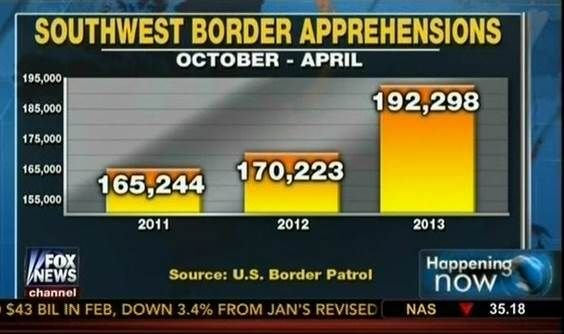
\includegraphics[width=3.75in]{../images/ch02_bad_nonzero}\par
\end{center}
\end{frame}

\begin{frame}{Non-zero axis, fixed}
\begin{center}
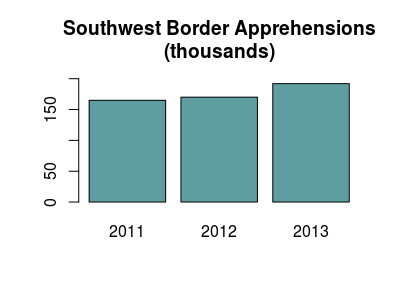
\includegraphics{../images/ch02_bad_nonzero_fixed} 
\end{center}
\end{frame}

\begin{frame}{Misleading graphs: pictographs}
\begin{block}{}
A \bt{pictograph} uses pictures or 3D objects to represent size, rather than simple bars or points. This can also distort relative sizes.
\end{block}

\pause
\begin{exampleblock}{Example}
Suppose we wanted to graph the difference in sales between two oil companies, one of which is has twice the sales as the other. If we created a pictograph, we would draw the height of the larger sales twice as tall as the other.
\begin{itemize}
\item If we used a pictures, such as a company logos, the larger would have 4 times the area.
\item If we used a 3D object, such as an oil barrel, the larger would have 8 times the volume. 
\end{itemize}
\end{exampleblock}
\end{frame}

\begin{frame}{Pictograph, example}
\begin{center}
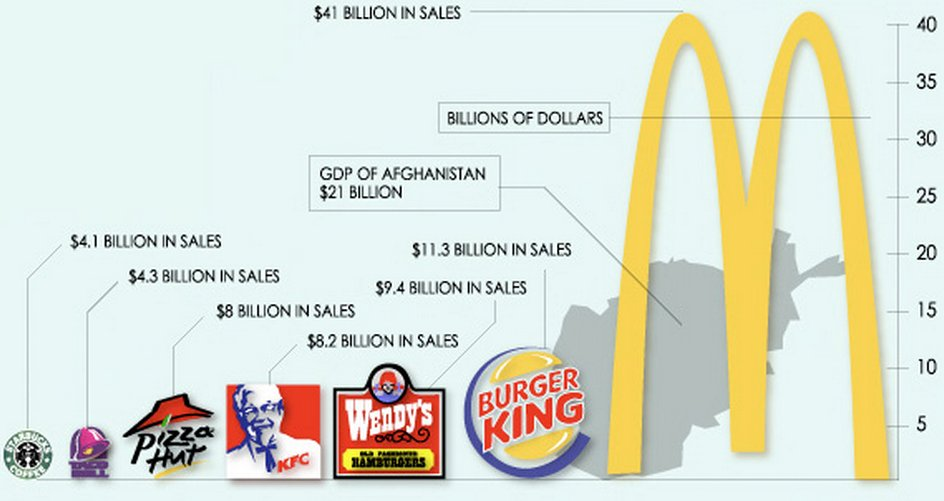
\includegraphics[width=4.5in]{../images/ch02_fastfood_pictograph}
\end{center}
\begin{block}{}
Note that KFC has twice the sales of Starbucks and McDonald's is about 4 times Burger King, but both differences appear much greater.
\end{block}
\end{frame}

\begin{frame}{Misleading graphs: pie chart abuse}
\begin{block}{}
Since pie charts represent portions of a whole, the slices should always\\ add up to 100\%.
\end{block}
\pause
\begin{center}
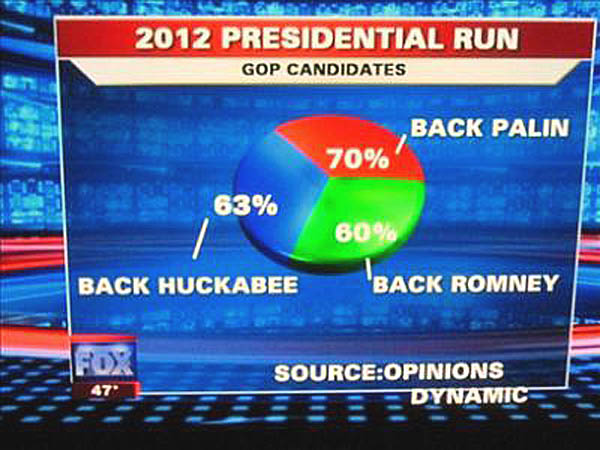
\includegraphics[width=3.2in]{../images/ch02_bad_piechart}
\end{center}

\end{frame}

\begin{frame}{No. Just no.}
\begin{center}
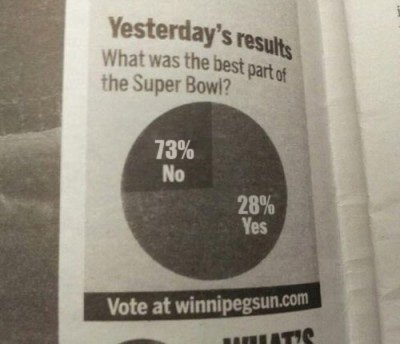
\includegraphics[width=3.5in]{../images/ch02_sb_piechart}
\end{center}
\end{frame}
\end{document}